\documentclass[titlepage,a4paper]{article}

\usepackage{a4wide}
\usepackage[colorlinks=true,linkcolor=black,urlcolor=blue,bookmarksopen=true]{hyperref}
\usepackage{bookmark}
\usepackage{fancyhdr}
\usepackage[spanish]{babel}
\usepackage[utf8]{inputenc}
\usepackage[T1]{fontenc}
\usepackage{graphicx}
\usepackage{float}
\usepackage{listings}
\usepackage[table,xcdraw]{xcolor}
\usepackage{listings}
\usepackage{amsmath}


\definecolor{codegreen}{rgb}{0,0.6,0}
\definecolor{codegray}{rgb}{0.5,0.5,0.5}
\definecolor{codepurple}{rgb}{0.58,0,0.82}
\definecolor{backcolour}{rgb}{0.95,0.95,0.92}

\lstdefinestyle{codestyle}{
    backgroundcolor=\color{backcolour},   
    commentstyle=\color{codegreen},
    keywordstyle=\color{magenta},
    numberstyle=\tiny\color{codegray},
    stringstyle=\color{codepurple},
    basicstyle=\ttfamily\footnotesize,
    size=1,
    breakatwhitespace=false,         
    breaklines=true,                 
    captionpos=b,                    
    keepspaces=true,                 
    numbers=left,                    
    numbersep=5pt,                  
    showspaces=false,                
    showstringspaces=false,
    showtabs=false,                  
    tabsize=2,
}


\lstdefinestyle{myListingStyle} 
    {
        basicstyle = \small\ttfamily,
        breaklines = true,
    }


\pagestyle{fancy} % Encabezado y pie de página
\fancyhf{}
\fancyhead[L]{Modelos y Optimización I (71.14) - Resumen}
\fancyhead[R]{Alvarez Windey Juan}
\renewcommand{\headrulewidth}{0.4pt}
\fancyfoot[C]{\thepage}
\renewcommand{\footrulewidth}{0.4pt}
\setlength{\arrayrulewidth}{0.5mm}



\begin{document}
\begin{titlepage} % Carátula
    
\includegraphics[width=12cm]{logofiuba.jpg}
    \centering
    \vfill
    \Huge  71.14 Modelos y Optimización I\\
    \vskip1cm
    \Huge 
    Resumen\\
    
    
    \large
    
    
    \vfill



\end{titlepage}

% Índice general
\tableofcontents

\newpage

\section{Pasos para plantear un problema en programación lineal}\label{sec:ej1}

\begin{enumerate}
    \item Escribir el objetivo (Qué hacer?, Cuándo? y Para qué?)
    \item Plantear las hipótesis
    \item Describir las variables de cantidades con sus unidades, ej: X: cantidad de x prod. [unidad/mes] (entera/continua)
    \item Plantear el modelo matemático:
    \begin{itemize}
        \item Describir cada una de las restricciones en palabras (si es de armado necesitara 1 restricción por elemento para el armado).
        \item Los únicos signos válidos en las restricciones son mayor o igual, igual o menor o igual. Todas las restricciones se tienen que poder convertir en igualdades para resolver el problema.
        \item Definir las variables de decisión (controlables)
        \item Expresar cada restricción en función de las variables de decisión
    \end{itemize}
\end{enumerate}


\vspace{0.5cm}

\subsection{Hipotesis y supuestos para los problemas}

\begin{itemize}
    \item No hay inflación ni varían los precios o costos
    \item No hay productos ni materia prima fallados
    \item No hay limitantes de recursos
    \item Todo lo que se produce se vende
    \item No hay desperdicio de recursos al fabricar
    \item Gastos de energía insignificantes
    \item Todos los parámetros del modelo son constantes conocidas (sirve para poder plantear el modelo dentro de la optimización deterministica)
    \item Hipótesis de proporcionalidad: tanto el beneficio como el uso de recursos son directamente proporcionales al nivel de actividad
    \item Hipótesis de aditividad: no existen interacciones entre las actividades que cambien la efectividad o el uso total de algún recurso.
    \item Hipótesis de divisibilidad: Las unidades de actividad pueden dividirse en niveles fraccionarios cualesquiera, de modo que pueden permitirse valores no enteros para las variables
\end{itemize}

\vspace{0.5cm}


\subsection{Variables}

\begin{itemize}
    \item Las variables slack o variables de holgura sirven para agregar un término positivo de un lado de una restricción esta se convierte en igualdad. Estás variables nos indicarán el sobrante de alguna variable.
    \item Continuas
    \item Enteras: productos enteros o recursos enteros
    \item Bivalentes o indicadoras (0,1): variables de decisión, señalan alternativas posibles o indicativas marcan el estado de una variable asociada
    \item Exceso y defecto: van juntas ya que no puede haber variables negativas 
\end{itemize}

\vspace{0.5cm}

\section{Tipos de problema}

\begin{itemize}
    \item Problemas de mezcla: Uso de porcentajes y cantidades no enteras. Se mezclan ciertos insumos para producir otros bienes a vender.
    \item Problemas de armado: Uso de cantidades enteras. A diferencia del problema de mezcla, en este caso el producto final sigue manteniendo la esencia de las partes que lo componen, no se forma algo original/diferente. En gral. en estos problemas se necesita una restricción por cada tipo de elemento que interviene en el armado de un producto.
    \item Problema de producción: Cuánto tengo que producir. La producción se divide en distintos lugares físicos en cada uno de los cuales se realizan distintas partes del proceso.
    \item Problema de multiperiodo: Tiene varios periodos, en el cual cada uno esta relacionado con el anterior y el siguiente
    \item Problema del viajante: Consiste en determinar el circuito más eficiente de un viajante que tiene que recorrer una serie de puntos
    \item Problema de distribución o transporte: Hay un conjunto de lugares que disponen de los suministros que son los orígenes y lo destinos que con los conjuntos de lugares a ser abastecidos 
    \begin{itemize}
        \item Problema del Transbordo: Los suministros no van a los destinos sino que van a un punto intermedio.
        \item Problema de asignación: es como el problema de transporte pero todas las demandas y ofertas son iguales a 1. Hay que encontrar los conjuntos (a, b) (siendo a origen y b destino) tal que minimice los costos
    \end{itemize}
    \item Problema de cobertura de conjuntos: Hay 3 tipos:
    \begin{itemize}
        \item Cobertura: se cubran todos los elementos de S con solapamiento ($\geq 1$).
        \item Partición: se cubran todos los elementos de S sin solapamiento ($= 1$).
        \item Packing: se cubra la máxima cantidad de elementos de S que se pueda sin solapamiento ($\leq 1$)
    \end{itemize}
    \item Problema de secuenciamiento de tareas (scheduling): cual es el orden más óptimo para realizar ciertas tareas
\end{itemize}

\vspace{0.5cm}

\subsection{Problemas de armado}

Las situaciones en las cuales se debe fabricar un producto utilizando determinada cantidad de otros productos (cantidades y no porcentajes) reciben el nombre de problemas de armado. A diferencia de los problemas de mezcla, los productos que intervienen en el armado no generan algo diferente, como en el problema de mezcla,
sino que siguen manteniendo su esencia original.

La única manera de avisarle algo al modelo es con restricciones. En el ejemplo que había del armado de muñecos la siguiente ecuación estaba MAL:

$$ (CABEZAFEMENINA + TORSOFEMENINO + PIERNA + BRAZO) / 6 = DAMA $$

Está MAL porque si DAMA vale 1 el modelo podría, con esta única restricción, darle el
siguiente valor a las variables:
CABEZAFEMENINA = 6, TORSOFEMENINO = 0, PIERNA = 0, BRAZO = 0 lo cual originaría un monstruo de 6 cabezas.
El mensaje que le damos al modelo es que para hacer un muñeco se necesitan 6 piezas de cualquier tipo, porque en la restricción sumamos todos los tipos de pieza y lo dividimos por 6.
Una característica de los modelos de armado es que se necesita una restricción por cada tipo de elemento que interviene en el armado de un producto. En el ejemplo de los muñecos sería:

$$ 1 (cabeza/muñeco) DAMA (muñeco/mes) = CABEZAFEMENINA (cabeza/mes) $$
$$ 1 (torso/muñeco) DAMA (muñeco/mes) = TORSOFEMENINO (torso/mes) $$
$$ 2 (brazo/muñeco) DAMA (muñeco/mes + 2 (brazo/muñeco) CABALLERO (muñeco/mes = BRAZO (brazo/mes)  $$
...

\vspace{0.5cm}

\subsection{Problema del viajante}

\begin{itemize}
    \item Se llama $C_{ij}$ a la distancia entre el punto i y j
    \item Viajante simétrico: no importa la dirección ($C_{ij} = C_{ji}$)
    \item Viajante asimétrico: importa la dirección
    \item $Y_{ij}$ vale 1 si el tour va de i a j, vale 0 en caso contrario
\end{itemize}


\textbf{Formulación matemática}

Al menos 1 camino llega hasta cada j

$$ \sum_{\substack{i=0 \\ i \neq j}}^{n} Y_{ij} = 1 ,\quad \forall j = 0 ,1 ,2 ...,n $$

Al menos 1 camino sale de i

$$ \sum_{\substack{j=0 \\ i \neq j}}^{n} Y_{ij} = 1,\quad \forall i = 0 ,1 ,2 ...,n $$


Funcional: 

$$ Z = \sum_{\substack{i=0 \\ j=0 \\ i \neq j}}^{n} C_{ij} Y_{ij} \quad (MINIMO) $$

Evitar "subtours" (que sea un único camino conexo):

\vspace{0.25cm}

$Ui$: Número de secuencia en la cual la ciudad i es visitada,  $\forall i = 1 ,2 ,3 .... ,n $ (variables \textbf{enteras})

$$ U_{i} - U_{j} + n Y_{ij} \leq n - 1 $$
$$ \forall i = 1 ,2 ,3 .... ,n $$
$$ \forall j = 1 ,2 ,3 .... ,n $$
$$ i \neq j $$

\textbf{Importante}:  las $Ui$ no se definen para la ciudad 0 (de origen y de partida) porque la idea de estas variables es que no se pueda ir de una ciudad que tiene un determinado número de orden (o de secuencia) a
una que tenga un orden menor. A la única que se puede volver es a la ciudad cero, porque no tiene este tipo de restricciones. Sin la ciudad cero (es decir, sin una ciudad que no tenga variable $Ui$ definida) el modelo no
funciona, porque la idea de este modelo es que arme un “arco” en el cual no se puede volver para atrás, por eso necesita una ciudad cero que esté fuera del arco.

Correlación Unitaria: El significado de las variables $Ui$ es el número de
secuencia en el cual es visitada la ciudad i. O sea si $Y_{ij} = 1 \implies U_{j} = U_{i} + 1$

Ejemplos: 
\begin{itemize}
    \item “No se puede visitar al cliente de la ciudad D si antes no se visitó al de la ciudad G”: $$UD \geq UG$$
    \item “No se puede visitar al cliente de la ciudad F si antes no se visitó al de la ciudad E o al de la ciudad B”: $$UF \geq UE - MY , \quad UF \geq UB - M (1 - Y)$$
\end{itemize}

\vspace{0.5cm}

\subsection{Problema de distribución o transporte}

Si todas las ofertas son números enteros y todas las demandas son números enteros, siendo todas las restricciones IGUALDADES, el problema de distribución o transporte tendrá como resultado que todas las variables tomarán valor entero aunque no se les ponga la condición de que las variables tienen que
tomar valor entero.
Por eso es que el problema de distribución o transporte se resuelve como un problema con variables continuas. Es muy importante que la oferta total sea igual a la demanda total (aunque sea agregando un origen ficticio o un
destino ficticio, según corresponda) para que se pueda verificar que resolviéndolo como continuo da resultado entero.

\vspace{0.25cm}

\textbf{Alternativa de transbordo}

Las variables serán:

$XOiTj$: cantidad de unidades que el origen i envía al transbordo j

$XTiDj$: cantidad de unidades que el transbordo i envía al destino j

\vspace{0.5cm}

\subsection{Cobertura de conjuntos}

Tendriamos distintos circuitos que cubren los distintos puntos. Ejemplo:

$$ Punto1) YA + YB + YE  \leq 1 $$

Si es cobertura el menor o igual sería mayor igual, si es partición sería igual y el caso que se muestra es el de packing.

\vspace{0.5cm}

\subsection{Problema de scheduling}

Se necesita saber el momento de inicio y de finalización de cada tarea, para ello se definen las siguientes variables:

$Iij$: Minuto en que empieza la tarea i en la máquina j

$Fij$: Minuto en el cual finaliza la tarea i en la máquina j

Si se quiere minimizar que tarea se termina antes se hace:

$$ Fij \leq FINAL \quad \forall i, j $$

$$ MIN \quad FINAL $$

Para que después no todas las tareas comienzen al mismo tiempo, habrá que indicarlo al modelo de la siguiente forma (tomamos una tarea A y B y una máquina "1"):

$$ FA1 \leq IB1 + M YanuloAB $$
$$ FB1 \leq IA1 + M (1 - YanuloAB) $$

Entonces por cada par de tareas en cada lugar se deberá incluir un par de variables





\newpage
\section{Programación lineal entera}

\subsection{Condiciones de vínculo}

Son las que relacionan las actividades entre sí o con el contexto.

\begin{itemize}
    \item Fuertes: deben ser cumplidas siempre.
    \item Débiles: pueden no cumplirse a un cierto costo (se resuelven con programación de metas).
    \item Conflictivas o contradictorias: dos o más condiciones no pueden cumplirse simultáneamente.
\end{itemize}

\vspace{0.5cm}


\subsection{Relaciones de AND y OR}

Se puede plantear un \textbf{and} de n variables binarias (n es una constante y es la cantidad de variables binarias que estamos sumando)

$$
n Y_{AND} \leq Y1 + Y2 + Y3 + Y4 + ... + Yn \leq (n - 1) + Y_{AND}
$$

También se puede plantear un \textbf{or} de n variables binarias:

$$
Y_{OR} \leq \sum_{i} Yi \leq n Y_{OR} 
$$

\subsection{Relación boleana con variables binarias indicativas}

Cuando se agrega la variable de producción como $Xi$, la variable binaria/decisión pasa a ser una variable indicativa. 

A diferencia de las variables de decisión, las variables indicativas necesitan restricciones para poder tomar el valor que indica su definición.

Por ejemplo: si tenemos $Xi$ como la cantidad de producto i que se fabrica y tenemos $Yi$ como variable para decidir si el producto i se fabrica o no,
Además de todas las restricciones deberíamos tener:

$$m Yi \leq Xi \leq M Yi$$

donde m es un número muy pequeño (cercano a cero) y M es un número muy
grande.

Esto se conoce como rangos de una variable

IMPORTANTE: Cuando se agrega la restricción del modelo bivalente a las restricciones se convierte en dos inecuaciones, una por cada signo mayor/menor

ej:
 
$$ 
2YAH < Y3 + Y4 < 1 + YAH \implies 2YAH - Y3 - Y4 \leq 0 \quad y \quad Y3 + Y4 - YAH \leq 1 
$$

\vspace{0.5cm}

\subsection{Metas}

Cuando queremos saber si una variable está por encima de otra, o bien para estar al tanto de una meta economica. Usaremos las variables EXCESO y DEFECTO. 

$$ X1 - X2 = EXCESO - DEFECTO $$

$$ m YEXCESO \leq EXCESO \leq M YEXCESO $$

$$ m YDEFECTO \leq DEFECTO \leq M YDEFECTO $$

$$ YEXCESO + YDEFECTO \leq 1 $$

La última ecuación impide que ambas sean igual a 1. 

Si queremos saber si son iguales podriamos hacer:

$$ YEXCESO + YDEFECTO + YIGUALES \eq 1 $$



\vspace{0.5cm}

\subsection{Eliminación de restricciones (Decisión de alternativas)}

Este puede ser un caso en que tengamos dos opciones distintas pero excluyentes una de otra, por lo que el termino M se multiplicaría por la correspondiente variable binaria de si se toma la decisión o no y luego se obligará a que las 2 variables binarias sumadas valgan 1 (así obligo al modelo a tomar una sola opción)

\vspace{0.5cm}

Si la restricción es de menor o igual el término independiente (3 + M) tiene que tener un valor muy grande para que la restricción no restrinja

$$ X1 + X2 \leq 5 $$
$$ X1 \leq 3 + M Y_{anulo} $$
$$ MAX Z = X1 + X2 $$

\vspace{0.5cm}

Si la restricción es de mayor o igual el término independiente (3 - M) tiene que tener un valor muy chico (cero o menor que cero) para que la restricción no restrinja

$$ X1 + X2 \leq 5 $$
$$ X1 \geq 3 - M Y_{anulo} $$
$$ MAX Z = X1 + X2 $$

\vspace{0.5cm}

\subsection{Costo de mantenimiento diferencial (Costo diferencial por intervalo)}

Si el costo varía según distintos intervalos, para evitar multiplicar una variable no binaria por una suma de varias binarias (NO LINEAL),
lo que hacemos es dividir la variable no binaria en tantos intervalos como necesitemos y asi multiplicar $(m Yi < Xi < M Yi)$ cada tramo por su variable binaria. Y no podrá haber varios de esos tramos activos al mismo tiempo → $Y1 + Y2 + ... + Yn = 1$.
Si la variable entera fuese cantidad de horas usadas en una máquina las restricciones quedarían:



$$ 1*YH1 \leq H1 \leq 30*YH1 $$

$$ 30,01 YH2 \leq H2 \leq 59,99 YH2$$  

$$60 YH3 \leq H3 \leq M*YH3$$

Restricción para que una sola variable se active

$$YH1 + YH2 + YH3 = 1$$

\textbf{Recordemos que NO se pueden poner restricciones de mayor o menor estricto}

Y el costo de mantenimiento será:
$$ COSTO = H1 + 0,7H2 + 0,5H3 $$

\textbf{Importante los números que multiplican son a modo de ejemplo.}

\vspace{1cm}

\subsection{Función cóncava seccionalmente lineal}

Este caso se da por ejemplo si el precio de venta de un producto va variando por tramos según unidades vendidas. La diferencia con el caso anterior
es que antes todas las variables enteras (pueden ser horas) tenían el mismo costo pero variaba según su cantidad total, acá el costo es por tramos. 
Entonces la variable de precio nos quedaría $Xi = Xia + Xib + ... + Xin$

Y para restringir los valores entre ellas creamos una estructura tipo "represa", nos quedarían los siguientes rangos (tomamos el ejemplo de solo 3 variables) :

$$ n YiB \leq XiA \leq n $$
$$ k YiC \leq XiB \leq k YiB $$
$$ XiC \leq M YiC $$


\vspace{1cm}


% \section{Óptimo en un gráfico de Programación Lineal continua}

% \begin{itemize}
%     \item Siempre son vértices del conjunto convexo que es solución, por lo que no vale la pena analizar
% algún punto que no sea un vértice
%     \item Para saber cuál es el punto óptimo podemos graficar la traza de la función objetivo (la línea).
%     \item Hay que desplazar esa traza del funcional desde el (0, 0) lo más lejos
% del (0,0) que se pueda (porque estamos maximizando) hasta que no
% podamos movernos más porque “se termina el poliedro”
% \end{itemize}

% \vspace{0.5cm}









\section{Método Simplex}

Es un procedimiento iterativo que permite ir mejorando la solución a cada paso. El proceso concluye cuando no es posible seguir mejorando más dicha solución.
Partiendo del valor de la función objetivo en un vértice cualquiera, el método consiste en buscar sucesivamente otro vértice que mejore al anterior. La búsqueda se hace siempre a través de los lados del polígono (o de las aristas del poliedro, si el número de variables es mayor). Cómo el número de vértices (y de aristas) es finito, siempre se podrá encontrar la solución.

El método del simplex se basa en la siguiente propiedad: si la función objetivo, f, no toma su valor máximo en el vértice A, entonces hay una arista que parte de A, a lo largo de la cual f aumenta.

\vspace{0.5cm}

\textbf{Pasos del método Simplex}


\begin{enumerate}
    \item Convertir las restricciones del problema a inecuaciones con el término independiente aislado en uno de los lados → $X1 + X2 + ... + Xn \leq K$
    \item Convertir las inecuaciones en una igualdad, agregando las variables slack correspondientes → $X1 + X2 + ... + Xn + SLACKCORRESPONDIENTE = K$
    \item Las slacks \textbf{no} pueden ser negativas, por lo que si hay restricciones de mayor o igual se deberá agregar \textbf{variables artificiales}
    \item Igualar la función objetivo a 0.
    \item Con las distintas ecuaciones armar el sistema matricial $Ax = b$, siendo A la matriz con coeficientes, X el vector con todas las variables + slacks y b el vector de términos independientes.
    \item Buscaremos las soluciones en los vértices (porque solo esas pueden ser las óptimas). La cantidad máxima de variables que pueden ser distintas de cero en un vértice es igual a la cantidad de restricciones que tiene el problema.
\end{enumerate}

\subsection{Variables artificiales}

Si al momento de plantear el método tenemos una restricción que es de mayor o igual, tal que: $X1 \geq 10$, además de restar la slack correspondiente para igualar la ecuación sumaremos una variable artificial para que \textbf{la slack no valga 0 en la primera iteración}, que no representará ningún recurso como lo hacen las demás slacks de recursos, pero que servirá para plantear el modelo en la primera iteración y deberá salir siempre fuera de la base cuando se halle el óptimo, caso contrario (si se encuentra en la base) estariamos frente a una solución no factible.
En el ejemplo de arriba nos quedará $X1 - Xslack + \mu = 10$

Para que no afecte en la variable objetivo se le asigna un coeficiente o muy grande o muy chico dependiendo el problema (siendo M muy grande ):

\begin{itemize}
    \item -M en problemas de maximización 
    \item +M en problemas de minimización
\end{itemize}

Un ejemplo sería:

$$Zmax = X1 +2X2 - M*\mu$$

Al ser un problema de maximización lo más seguro es que el modelo no contenga en la base a la variable artificial ya que le resta mucho a el funcional.

\vspace{0.5cm}

% \subsection{Casos en un problema de PLC}

% Cuando se resuelve un modelo y se trata de hallar un óptimo puede suceder una de las siguientes cosas:

% \begin{itemize}
%     \item Tiene una solución óptima única
%     \item Tiene una cantidad finita de soluciones óptimas (soluciones alternativas óptimas). Este caso se identifica de manera gráfica cuando la traza de la función objetivo coincide con un lado del poliedro óptimo
%     \item No es factible (INCOMPATIBLE → NO HAY POLIEDRO). No se puede formar la región de soluciones factibles
%     \item Es no acotado. Esto se da solo en un modelo de maximización. Hay puntos con valor de Z arbitrariamente grande en la región factible (POLIEDRO ABIERTO)
% \end{itemize}

% \vspace{0.5cm}
 
\subsection{Búsqueda de vértices}


El primer vértice sería cuando todas las variables valen 0, posicionándonos en el vértice del origen, por lo que las variables slacks tomarían el máximo de su valor, esto nos da la ventaja de que los vectores de las variables distintas de cero son canónicos distintos (las variables que se encuentran en la columna X además se las llamas \textbf{variables base}: Si son productos indica cuanto se produjo, y si son recursos indica cuanto sobro, y si no están en la base indican lo contrario) y, por lo tanto, linealmente independientes (necesario para esto).
Lo siguiente es armar una tabla tal que:

\begin{figure}[H]
    \centering
    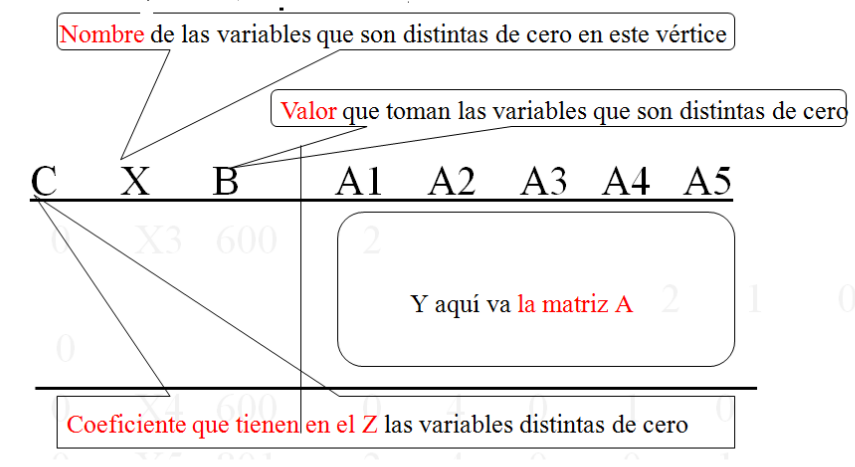
\includegraphics[scale=0.5]{tabla_simplex.png}
    \caption{Tabla Método Simplex}
\end{figure}


→ Si tomamos el ejercicio de la heladería del PDF (9.1) nos quedaría la siguiente tabla

\begin{figure}[H]
    \centering
    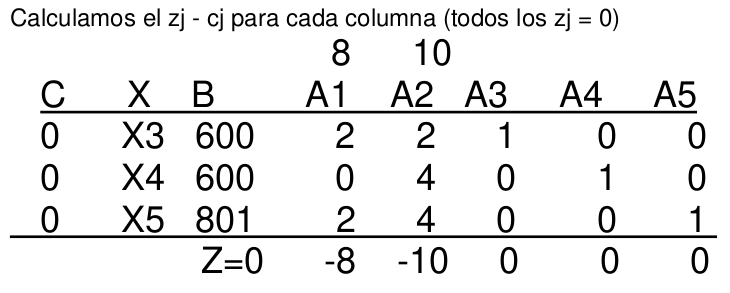
\includegraphics[scale=0.5]{primera_tabla_simplex.png}
    \caption{Primera Tabla Método Simplex}
\end{figure}

Como hay dos $zj - cj$ negativos (al ser el directo) aún \textbf{no hemos llegado al óptimo} (si es negativo es que no se llego al óptimo), para llegar al óptimo se debe cumplir que $zj - cj \geq 0 \quad \forall j$ .

La fórmula para los $Zj$ son:

$$Zj = C x Aj$$

Siendo C \textbf{TODO} el vector de coeficientes de variables que se encuentran en la base. Ahora entonces $Zj - Cj$ nos quedará:

$$Zj - Cj = C x Aj - Cj$$

En el ejemplo tenemos:
$$ Z1 - C1 = 2*0 + 0*0 + 2*0 - 8 $$
$$ Z1 - C1 = 2*0 + 4*0 + 4*0 - 10 $$

Para elegir que variable debe \textbf{ENTRAR} a la base, tenemos que elegir todas las variables cuyo $Zj - Cj$ sea menor que cero. Para decidir que variable debe \textbf{SALIR} de la base lo que conviene hacer es calcular el menor coeficiente $\theta$, que este coeficiente se calcula:

$$ \theta = \frac{Bi}{Aji} $$

Como $\theta \geq 0$ $\implies$ $\theta$ cuya $Aij \leq 0$ no se calculan 

\begin{figure}[H]
    \centering
    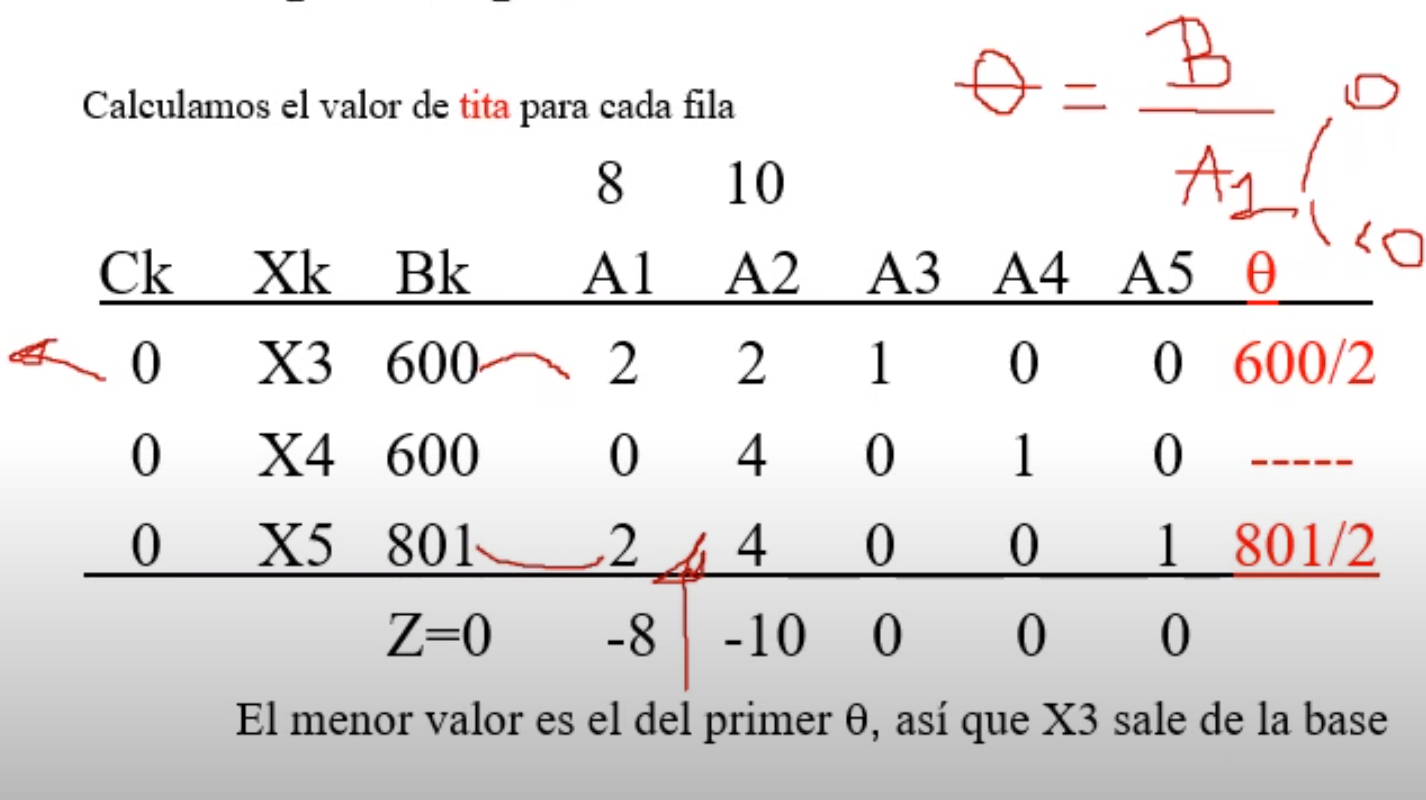
\includegraphics[scale=0.33]{tabla_simplex_theta.png}
    \caption{Tabla Simplex Theta}
\end{figure}


Cuando calculamos los $\theta$ nos quedamos con el mínimo, por lo que la variable que corresponde a ese $\theta$ saldrá de la base

Luego de elegir que variable entra a la base y cual sale, hay que cambiar de base. Para cambiar de base se seguirán los siguientes pasos:

\begin{enumerate}
    \item Elegir el elemento pivote, que está en la base (X3 para el ej) con la columna de la variable que entra a la base (X1 para el ej)
    \item Dividir la fila del pivote por el valor del pivote
    \item Completar la columna del pivote con ceros.
    \item Aplicar la regla del pivote que veremos a continuación para obtener el resto de valores (\textbf{para los $Bi$ también va esta formula})
\end{enumerate}


\begin{figure}[H]
    \centering
    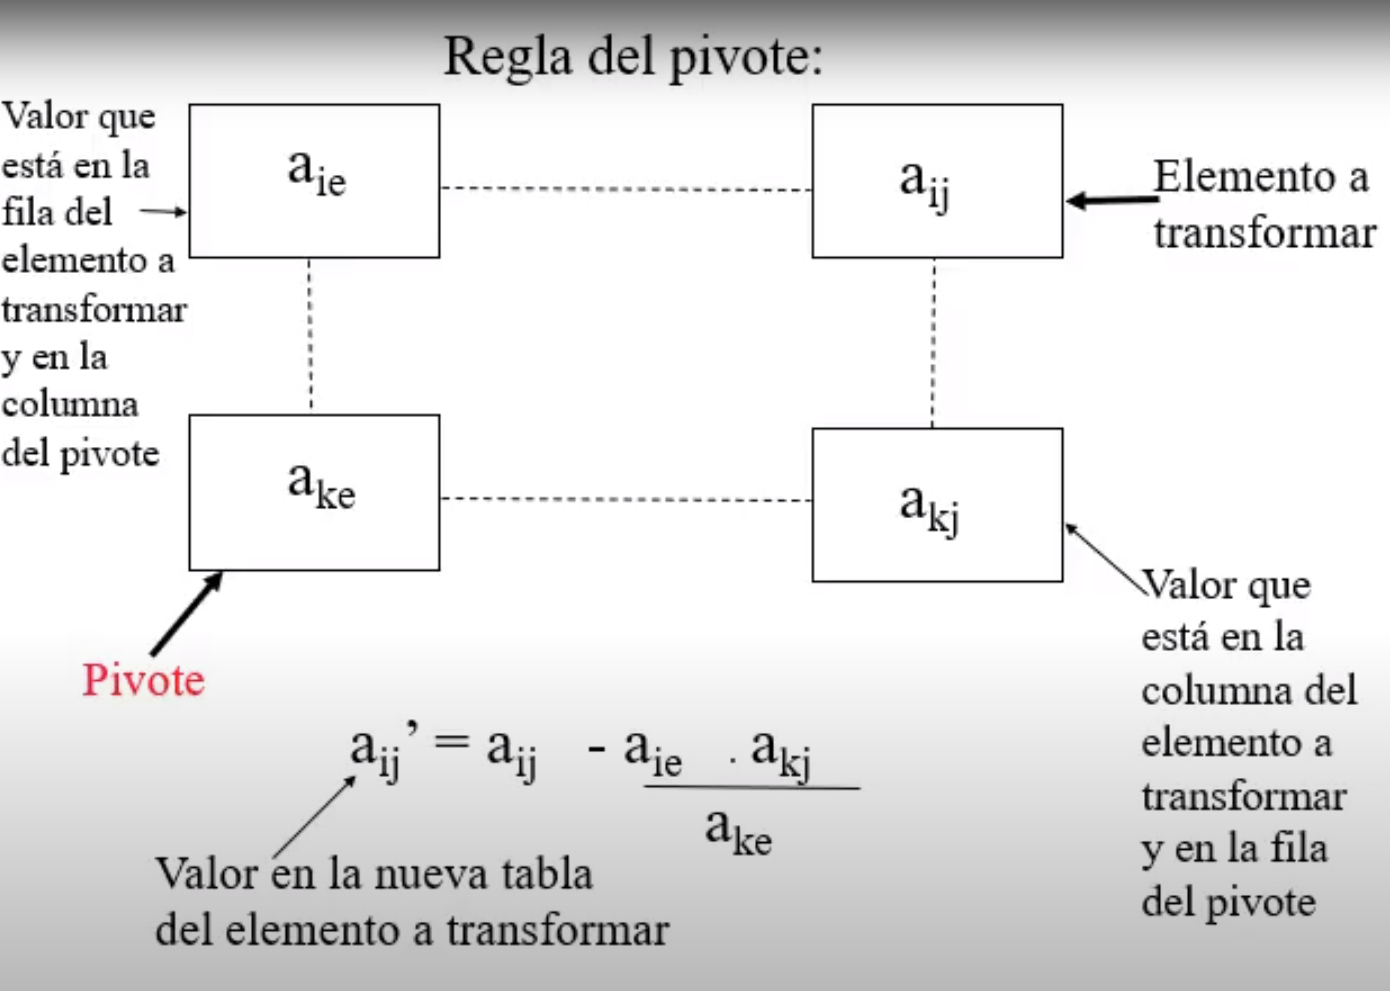
\includegraphics[scale=0.30]{regla_pivote.png}
    \caption{Regla pivote}
\end{figure}

Aca podemos ver porque $\theta \geq 0$

La \textbf{fila} que corresponde a donde esta el pivote, se divide toda por el valor del pivote (ya tiene que quedar igual a 1), y la \textbf{columna} tendrá todos ceros menos un 1 en el lugar del pivote (ya que pertenecerá a la base)

Entonces luego de esto (para el ejemplo) la segunda tabla nos quedará de la siguiente forma:

\begin{figure}[H]
    \centering
    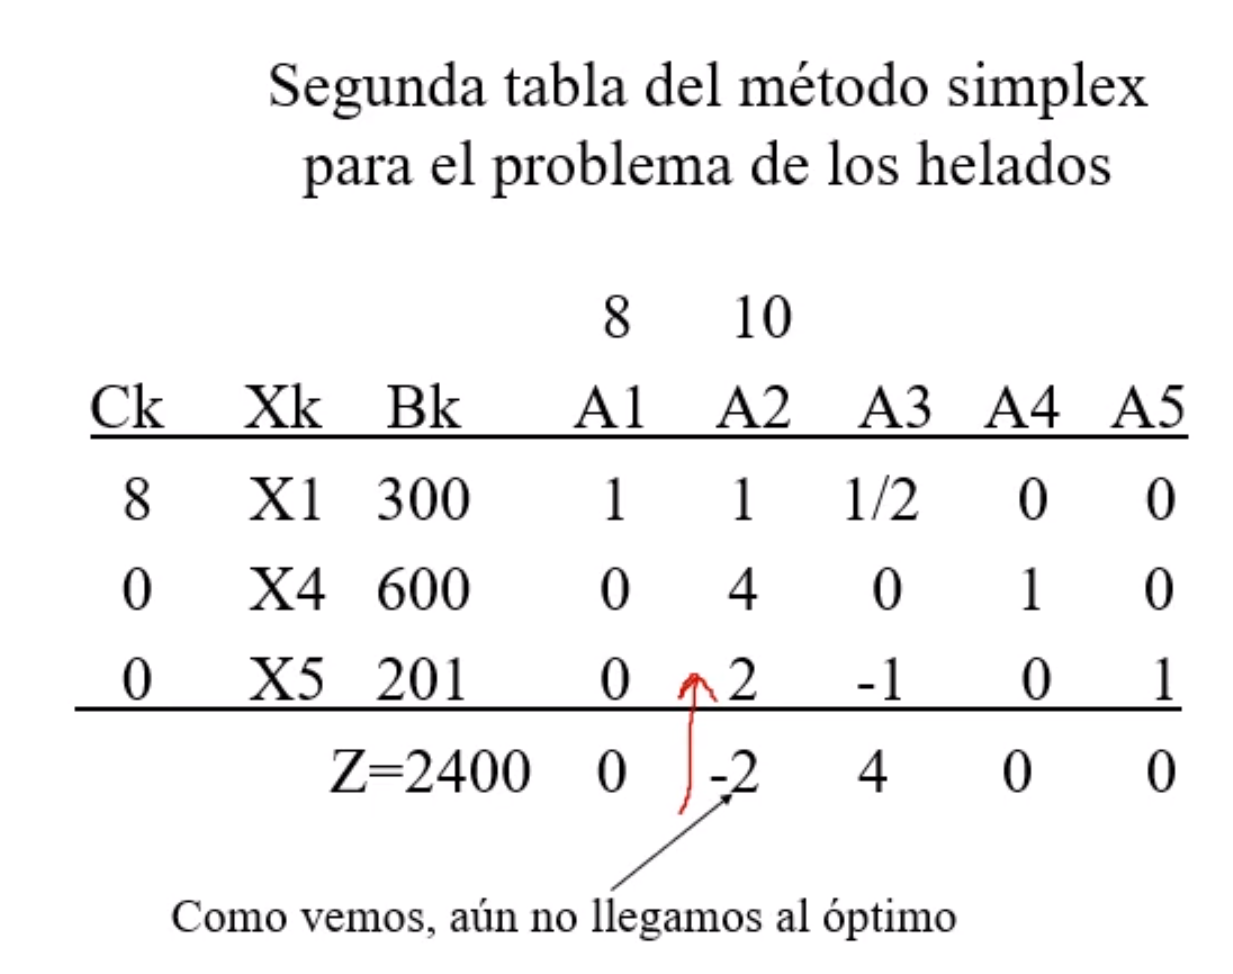
\includegraphics[scale=0.33]{segunda_tabla_simplex.png}
    \caption{Tabla simplex segunda tabla}
\end{figure}


Luego de esto repetimos el proceso hasta llegar al óptimo

\textbf{IMPORTANTE}: Recordar que para calcular el funcional de la tabla hay que multiplicar los vectores $C x B$. En este caso por ejemplo es:

$$ Z = 8 * 300 + 0 * 600 + 0 * 201 = 2400 $$ 

\vspace{1cm}

\subsection{Valor marginal y Costo de Oportunidad}

\begin{itemize}
    \item Los recursos que están saturados son los que no se hayan en la base a la hora de hallar la tabla óptima →
    \begin{itemize}
        \item Qué pasa si consigo más cantidad de un recurso saturado? gano más?
        \item Qué pasa si me obligan a fabricar más de un producto? desmejora el funcional?
        \item Qué pasa si la restricción se \"afloja\"? ganó más?
    \end{itemize}
\end{itemize}


\subsection{Costo de oportunidad}

\begin{itemize}
    \item Si el $zj - cj$ corresponde a una variable real del problema (por lo general representa productos fabricados) se llama \textbf{costo de oportunidad} (\textbf{CO}) de ese producto  (En LINDO se llaman \textbf{reduced cost})
    \item El costo de oportunidad es distinto de cero cuando la variable correspondiente al producto no está en la base (porque vale 0). Por que, si nos obligan a producir alguna unidad de algo que ya no estamos produciendo (dado que no conviene) el funcional empeorará
    \item El costo de oportunidad de un producto indica en cuánto va a desmejorar el funcional si tenemos la obligación de fabricar una unidad de ese producto
\end{itemize}

\vspace{0.5cm}

\subsection{Valor Marginal}


\begin{itemize}
    \item Si el $zj - cj$ corresponde a una variable slack del problema (por lo general representa sobrantes de recursos) se llama \textbf{valor marginal} (\textbf{VM}) de ese recurso o restricción (En LINDO se llaman \textbf{dual prices})
    \item El valor marginal es distinto de cero cuando la variable correspondiente al sobrante de recurso o slack de la restricción no está en la base (porque vale 0). Por lo que claramente, al no estar en la base, si conseguimos más de ese recurso limitado el funcional mejorará.
    \item El valor marginal indica en cuánto va a mejorar el funcional si esa restricción se afloja en una unidad. Si la restricción es menor o igual aflojar es aumentar el término indep., si la restricción es mayor o igual, aflojar es reducir el término indep.
\end{itemize}

\vspace{1cm}


\subsection{Dual}

\begin{figure}[H]
    \centering
    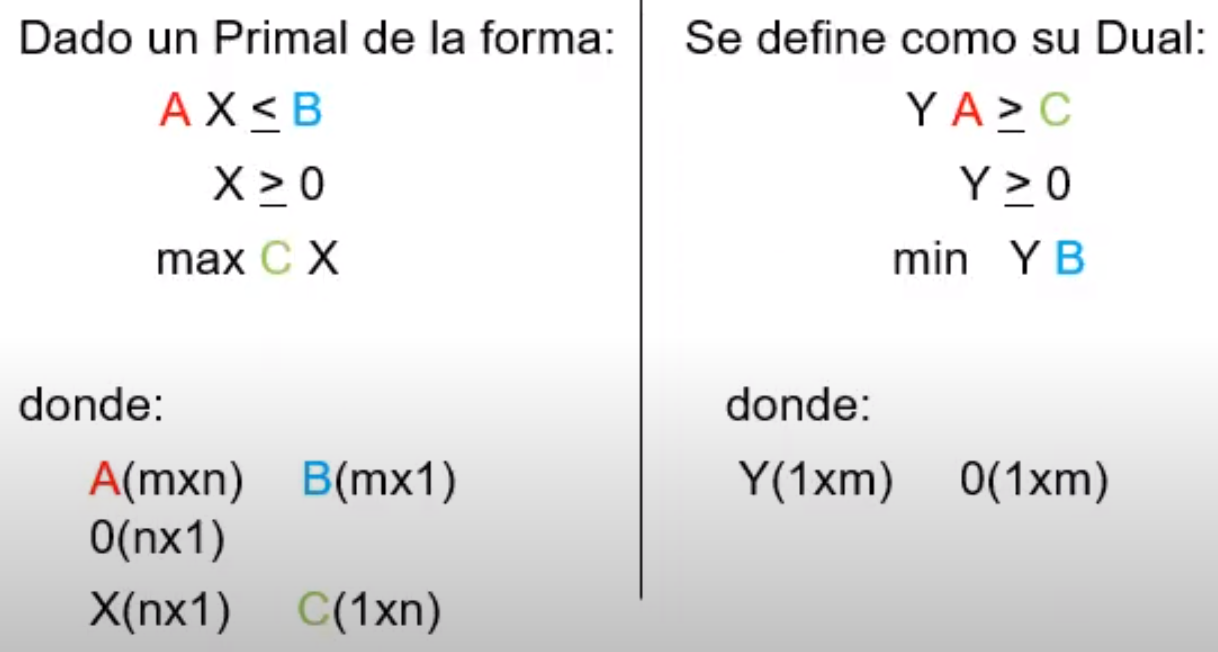
\includegraphics[scale=0.4]{planteo_dual.png}
    \caption{Planteo Dual}
\end{figure}

\begin{itemize}
    \item El dual tiene una variable real por cada restricción del problema primal
    \item El dual tiene tantas restricciones como variables reales tiene el primal
    \item El dual de un problema de maximización es un problema de minimización y viceversa
    \item Los coeficientes del funcional (costo o beneficio) del primal, son los términos independientes de las restricciones del dual
    \item Los términos independientes de las restricciones del primal son los coeficientes del funcional del dual
    \item Solo puedo pasar del directo al dual y viceversa, en la primera y en la tabla final (la óptima)
    \item \textbf{IMPORTANTE}: Si en un primer momento tenemos ecuaciones del tipo $X1 > 3$, habría que multiplicarlas por $-1$ y así obtener $-X1 < -3$, luego de hallar el óptimo del directo con esa forma, recién ahí se podría pasar al dual
\end{itemize}


Nuestro dual para el ejemplo anterior quedará de la siguiente forma:

\begin{figure}[H]
    \centering
    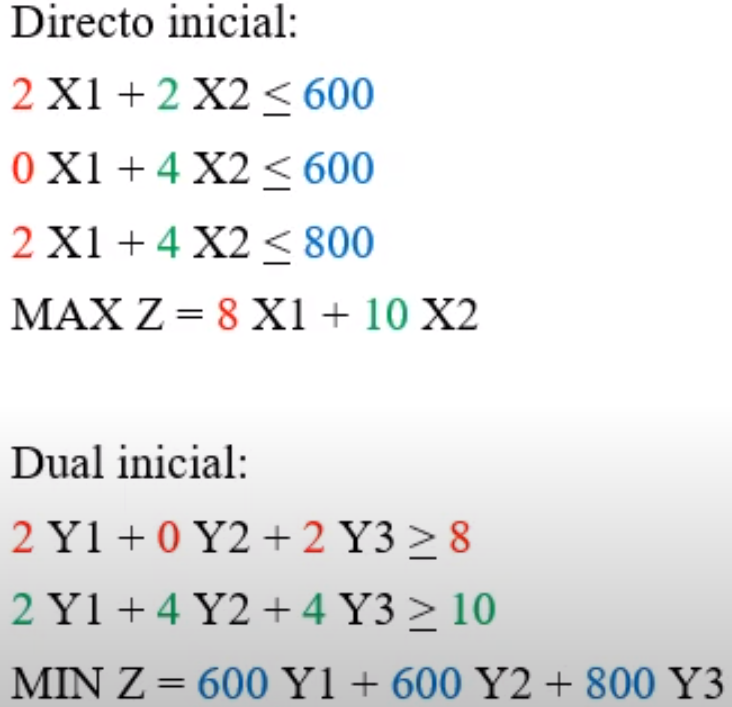
\includegraphics[scale=0.5]{dual_ejemplo.png}
    \caption{Dual ejemplo}
\end{figure}


\vspace{0.5cm}

\subsection{Teorema fundamental de la dualidad}
 

\textbf{TEOREMA}: Si el problema primal (o el dual) tiene una solución óptima finita, entonces el otro problema tiene una solución óptima finita, y el valor de los dos funcionales óptimos es el mismo

\begin{itemize}
    \item Si cualquiera de los 2 problemas tiene una solución óptima no acotada entonces el otro problema no tiene soluciones posibles
    \item Si cualquiera de los dos problemas tiene un punto degenerado entonces el otro problema tiene solución alternativa
\end{itemize}

→ \textbf{Solución óptima no acotada}: Se puede deber a un modelo mal construido, y se da con un problema de maximización. Tendríamos una región factible de soluciones infinitamente grande

→ \textbf{Solución no factible}: Se puede deber a un modelo mal construido, si alguna variable artificial nos queda en la base estaremos en este tipo de problema. No tenemos una región factible de soluciones

→ \textbf{Punto degenerado}: Sucede cuando más de dos rectas cortan en el mismo punto. Si quitamos alguna de las restricciones, la región de soluciones factibles sigue siendo la misma. En el método simplex sabremos que tendremos una solución degenerada si en algún paso previo a la obtención del óptimo podemos elegir entre 2 variables para que salgan a la base (ya que su $\theta$ da igual)

→ \textbf{Soluciones alternativas}: Sucede cuando la función objetivo es paralela a una restricción obligatoria no redundante. En el método simplex se dará cuando habiendo llegado a la tabla óptima, se pueda elegir para que una variable que no este en la base entre en ella, ya que su $Zj - Cj$ es igual a 0



\vspace{0.5cm}

\subsection{Teorema de la holgura complementaria}

Dados el problema primal y el dual correspondiente, siempre que en la k-ésima restricción de uno de ellos la variable de holgura o slack tome valor distinto de cero, entonces la k-ésima variable del otro problema desaparece de la base, y si la k-ésima variable de uno de los dos problemas es mayor que cero, en la k-ésima restricción del otro problema se verifica la igualdad (la variable slack o de holgura de esa restricción es igual a cero.

En el ejemplo:

\vspace{0.5cm}


\begin{tabular}{|l|l|}
\hline
\rowcolor[HTML]{EFEFEF} 
\multicolumn{1}{|c|}{\cellcolor[HTML]{EFEFEF}\textbf{PRIMAL}} & \multicolumn{1}{c|}{\cellcolor[HTML]{EFEFEF}\textbf{DUAL}}\\ \hline
X1 = 200 & Y4 = 0 \\ \hline
X2 = 100 & Y5 = 0 \\ \hline
X3 = 0   & Y1 = 3 \\ \hline
X4 = 200 & Y2 = 0 \\ \hline
X5 = 0   & Y3 = 1 \\ \hline                     
\end{tabular}


\vspace{0.5cm}

\subsection{Análisis de sensibilidad: Modificación de la solución óptima}


\subsubsection{Rango de variación de coeficientes de eficiencia (Cj)}


$\bullet$ Para realizar estos cambios en los coeficientes de eficiencia deben realizarse de a uno por vez

$\bullet$ Para realizar estas variaciones lo que conviene hacer es parametrizar los $cj$ y recalcular los $zj - cj$

\begin{figure}[H]
    \centering
    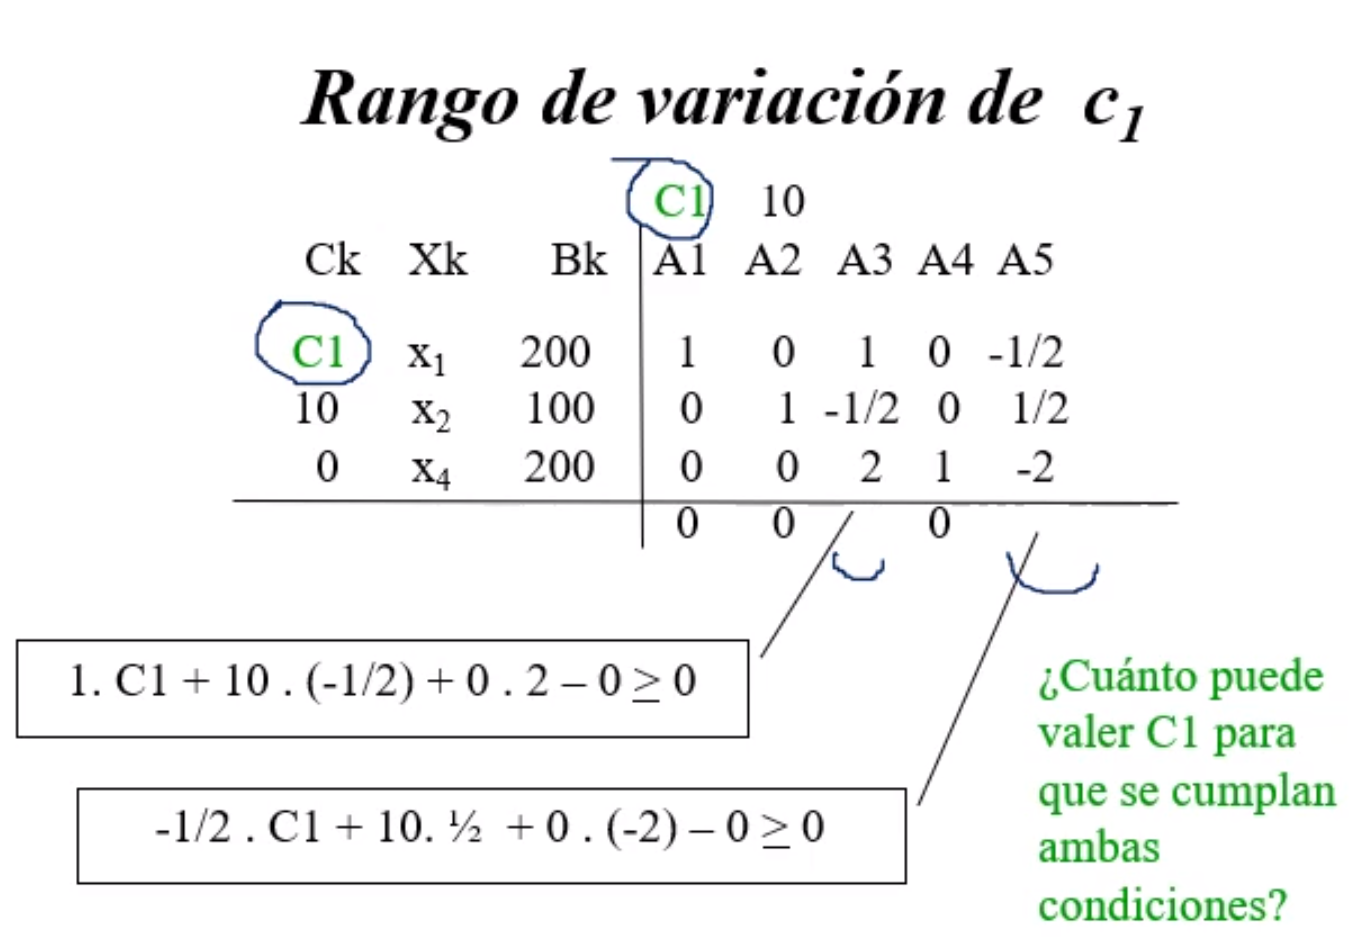
\includegraphics[scale=0.36]{parametrizacion_de_cj.png}
    \caption{Parametrizacion de Cj}
\end{figure}

$\bullet$ Una vez parametrizamos obtenemos los nuevos $zj - cj$ con el $cj$ parametrizado vemos en que punto dejan de valer cero, o lo que es lo mismo en que punto la tabla deja de ser óptima

$\bullet$ Recordar que si varío algún $Cj$ el valor del funcional \textbf{SI va a cambiar}, lo que no cambia es la base que forma parte de la solución óptima, dicho de otra forma el valor de las variables (lo producido y lo sobrante).

\vspace{0.5cm}

\subsection{Rango de variación de los términos independientes}

Una vez que tenemos el dual, podemos parametrizar los términos independientes de la misma manera que lo hicimos con los coeficientes de eficiencia

A su vez también se puede hacer el gráfico de “curva de oferta” pero de los valores marginales de las slacks, cambiando los valores que nos dan en los límites cuando parametrizamos el $zj-cj$

\vspace{1cm}

\subsubsection{Curva de oferta y gráfico del valor marginal}

\begin{itemize}
    \item La curva de oferta representa a los distintos valores que puede tomar el coeficiente $cj$ de un producto en el $Xj$, qué cantidad de ese producto $Xj$ es conveniente fabricar
    \item Para empezar la curva de oferta conviene empezar por la tabla óptima e ir variando los coeficientes e ir viendo los distintos intervalos (en los extremos de los rangos hay soluciones alternativas óptimas)
    \item Para la curva de oferta tendremos un gráfico continuo de a tramos y \textbf{creciente}, y para el gráfico de la variación del valor marginal (que se ve desde el dual) tendremos un gráfico continuo de a tramos y \textbf{descendiente}
\end{itemize}

\vspace{0.5cm}


\subsection{Variación simultanea de 2 recursos}

$\bullet$ Se presenta la posibilidad de conseguir azúcar entregando a cambio crema (para conseguir 1kg. de azúcar se deben entregar 1,5kg. de crema). Conviene?

Como son disponibilidades de recursos nos conviene trabajar en el dual, entonces nos quedaría asi la tabla:

\begin{figure}[H]
    \centering
    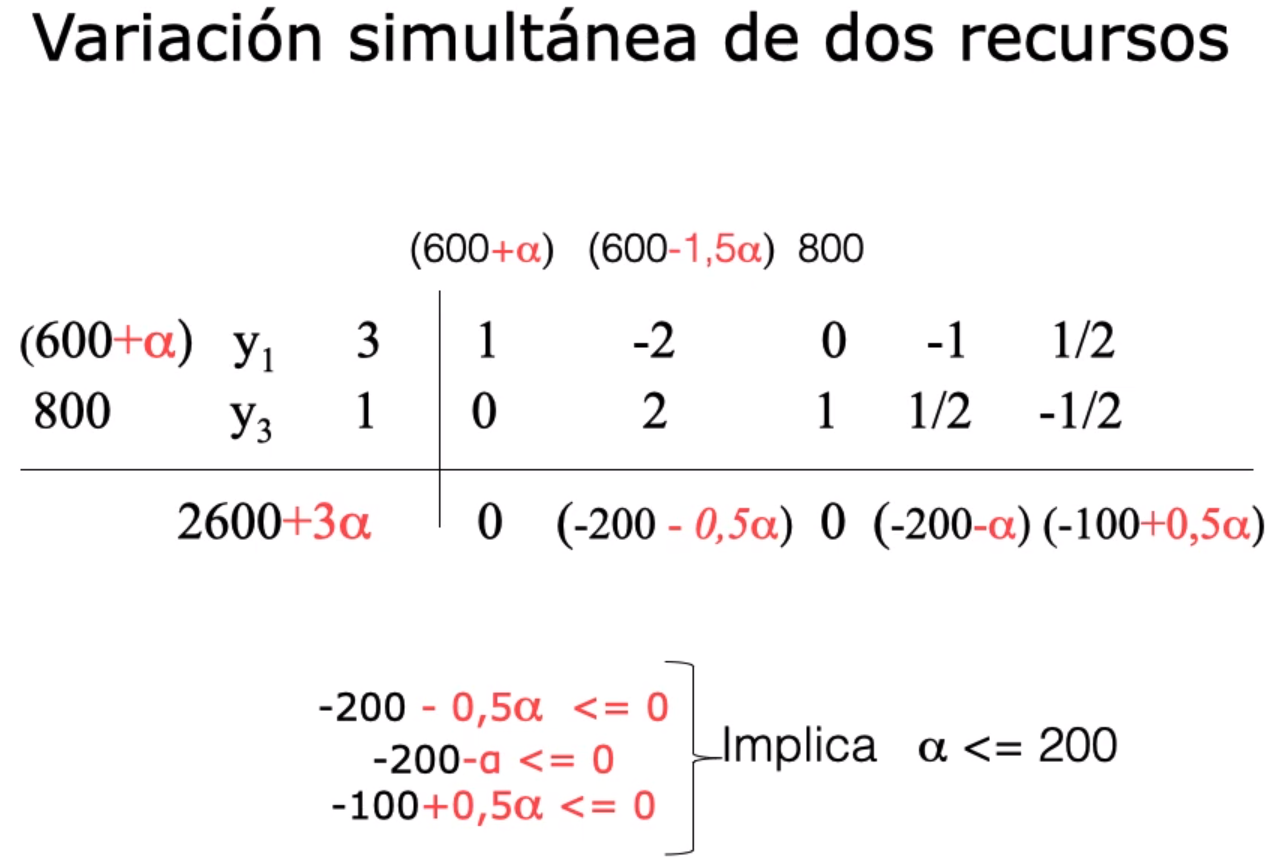
\includegraphics[scale=0.36]{variacion_simultanea.png}
    \caption{Variación simultanea}
\end{figure}

\vspace{0.5cm}

\subsection{Introducción de un producto adicional}

Qué pasa si queremos agregar un producto cuando ya tenemos la tabla óptima? Veamos las siguientes tablas:

\begin{figure}[H]
    \centering
    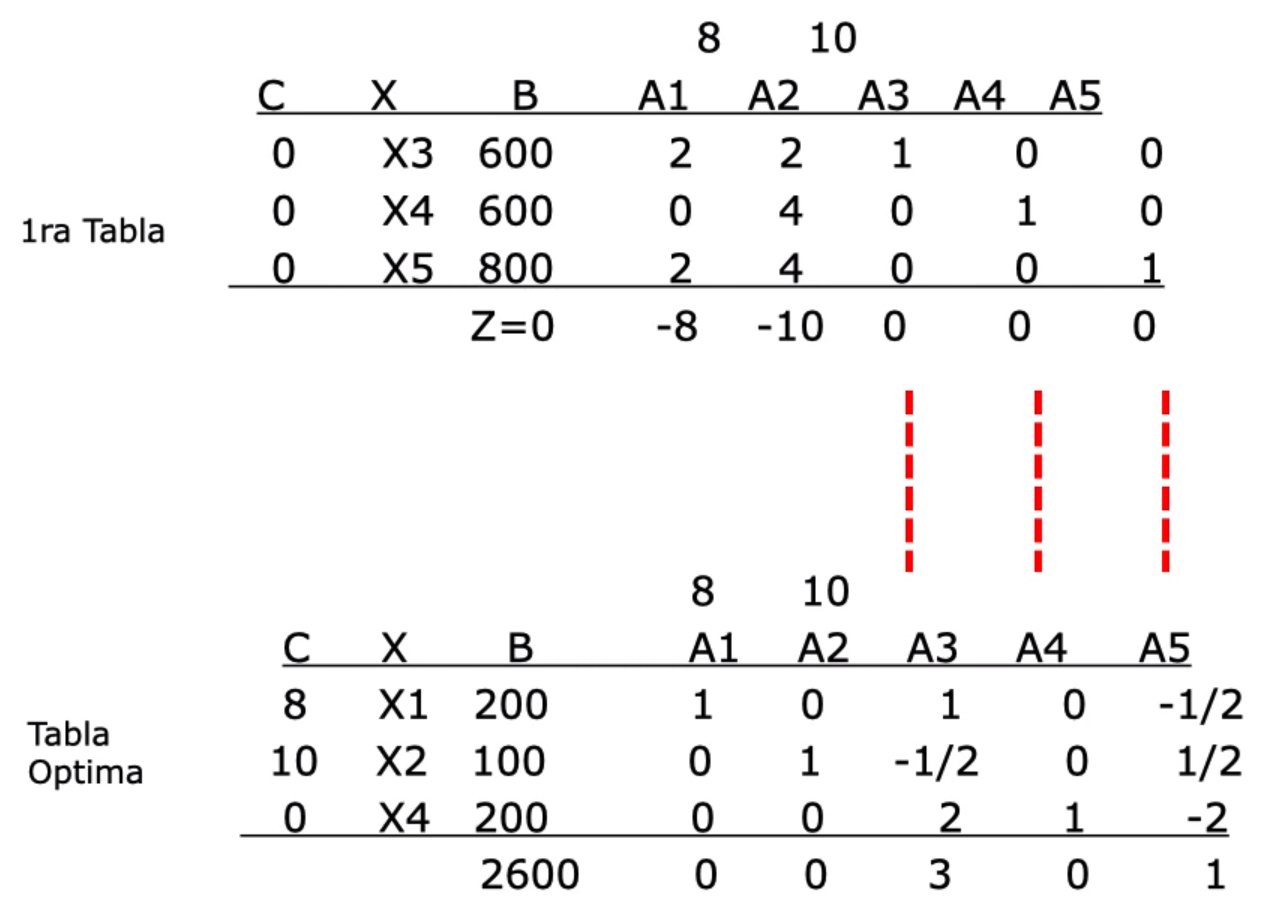
\includegraphics[scale=0.36]{matriz_inversa.png}
    \caption{Matriz inversa}
\end{figure}


La submatriz que se encuentra dentro de la tabla óptima y es la submatriz que se encuentra debajo de las 3 líneas rojas (de 3x3) es la matriz inversa de cambio de base.
Por ende si yo quiero agregar un nuevo producto, con sus correspondientes gastos de cada recurso $\implies$ lo que debo hacer es multiplicar a ese vector por la matriz inversa, y esa columna que nos da, será la que entrará en la tabla óptima. Luego, dependiendo de su $zj - cj$ podremos ver si aún nos encontramos en la tabla óptima, sino habrá que hallarla.

Algo importante a tener en cuenta, si una de las columnas de la matriz cambio de base corresponde a una variable artificial, entonces a esta habrá que cambiarle el signo antes de multiplicar el vector correspondiente al nuevo producto.

Por ejemplo, si queremos agregar un nuevo producto que consuma: 2kg de azúcar, 3kg de crema y 1kg de almidón por unidad, entonces la tabla nueva nos quedaría:


\begin{figure}[H]
    \centering
    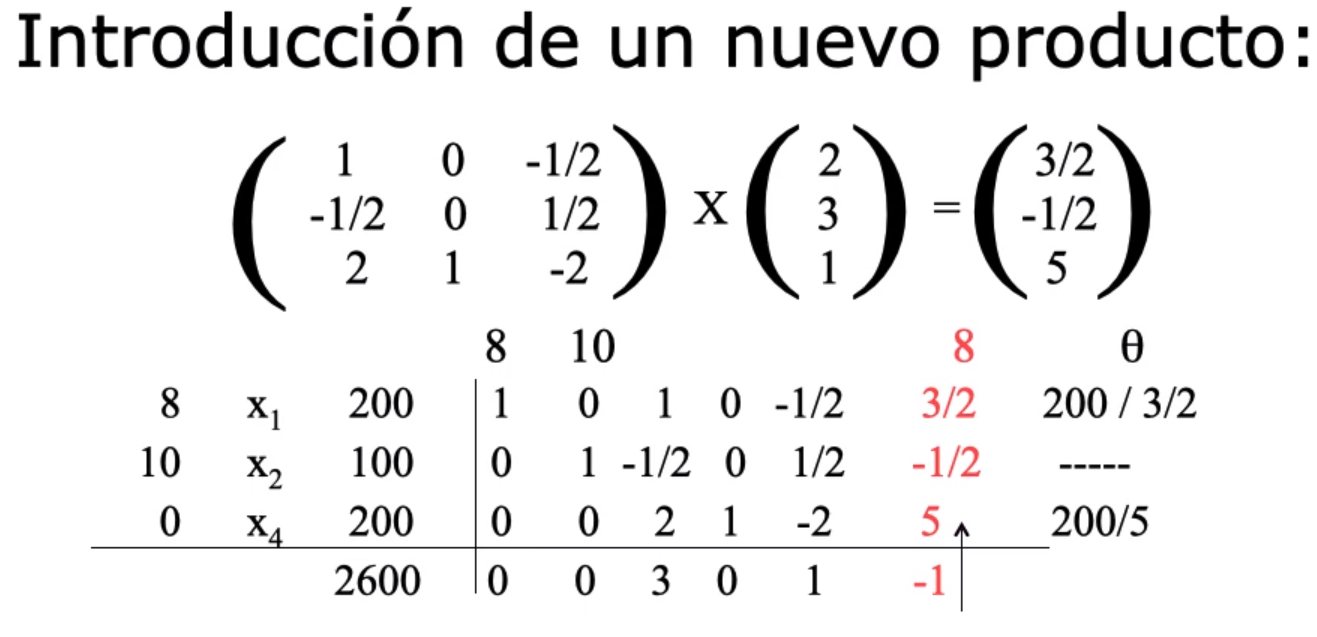
\includegraphics[scale=0.36]{nuevo_producto.png}
    \caption{Nuevo producto}
\end{figure}

Como podemos ver la nueva tabla no es óptima, por lo que habría que hallarla de nuevo

Si el agregado de la nueva restricción no me obliga a cambiar el directo óptimo, entonces quiere decir que la inclusión de ese nuevo producto no me aporta nada y/o no me conviene

\vspace{0.5cm}\vspace{0.5cm}

\subsection{Introducción de inecuaciones} 

\vspace{0.5cm}

La respuesta es sencilla, hay que trasladarse al dual y actuar como si quisiéramos agregar una nueva variable con la diferencia que la matriz inversa es importante tener en cuenta que probablemente las columnas que se encontraban en la base inicial en este caso eran variables artificiales (generalmente pasa si el directo es de max. y el dual de min.) por lo que habrá que \textbf{cambiarle el signo} a las columnas que correspondan a variables artificiales. Recordar que el dual es el directo transpuesto

Si el agregado de la nueva restricción no me obliga a cambiar el dual óptimo, entonces quiere decir que esa inclusión de recurso no me aporta nada y/o no me conviene

\vspace{1cm}

\subsection{Análisis de un problema de simplex} 


\begin{itemize}
    \item Comprar recursos: tendremos que ver si el costo a que se compran es menor que el valor marginal del mismo por la cantidad de unidades a comprar. Si multiplicamos las X unidades a comprar por el valor marginal obtendremos las \textbf{ganancias máximas} ya que habría que hacer el rango de variación en el dual del coeficiente $Cj$ (es útil para una primera aproximación) ya que a medida que \textbf{más} tengo de un recurso su valor marginal baja.
    \item Vender recursos: tendremos que ver que el valor de venta sea superior al valor marginal del recurso por la cantidad de unidades a vender. Si multiplicamos las X unidades a vender por el valor marginal obtendremos las \textbf{perdidas mínimas} ya que habría que hacer el rango de variación en el dual del coeficiente $Cj$ (es útil para una primera aproximación) ya que a medida que \textbf{menos} tengo de un recurso su valor marginal baja.
    \item Compra de recurso con demanda mínima: para ver si conviene nos tenemos que fijar el valor de venta sumado con el valor marginal de la slack de demanda mínima asociada (así podemos ver lo que ganamos con recursos liberados). Si tenemos la opción de comprar más de una unidad, nuevamente hacemos el rango de variación de la slack en el dual.
\end{itemize}

\vspace{1cm}

\section{Heurística (de construcción)}

\begin{itemize}
    \item Es una aproximación más "barata" para resolver un problema de PLC, que como veníamos haciendo con las inecuaciones.
    \item Son de orden polinomial (los de antes eran de orden exponencial). Por ejemplo cuando hay 2 ciclos for anidados 
    \item La heurística tiene que cumplir con las restricciones del modelo
    \item Tiene que tener una condición de corte clara y no caer en loops infinitos
    \item Indicar que hacer en desempates (Por ejemplo si se hace un índice/ranking de prioridades)
\end{itemize}
 

\end{document}
